\section{New Overview}
\label{sec:overview}
\hl{Pick an example}

\hl{explain what it does and why you should care about it}

\hl{Show how existing tools don't handle the example (to the best of our knowledge)}

\hl{Step through how Lakeroad handles the example.}

\hl{The rest of this paper details how Lakeroad generalizes all of these steps.}

\hl{At the end of overview: make the point that, you can use the same sketch for different workloads, and you can use the same sketch for workloads on different architectures.}

% Now, we will describe
%   the state of the art
%   synthesis tool for Xilinx FPGAs
%   compiles \texttt{((a+b)*c)\&d} onto
%   a Xilinx FPGA.

How does a user map a design to a DSP?
Let's consider the Xilinx DSP48E2,
  which implements any expression (design) of the form
  $((a \pm b) * c) \odot d$,
  where $\odot \in \{\land, \lor, \!\, \pm, \oplus \}$.
If a user wants to map the design
  \hl{include bitwidth and pipeline stages}
  $((a+b)*c) \:\&\: d$ to their DSP,
  ideally,
  they write the high-level behavioral Verilog
  shown in Figure~\cref{somefigure}.
\hl{figure to show the ``simple'' behavioral verilog}
  and pass that Verilog
  to an FPGA hardware synthesis tool.
Unfortunately,
  the state-of-the-art hardware synthesis tool
  for Xilinx FPGAs
  will fail to map the above design
  to a single DSP.
Furthermore, note that we include an annotation \texttt{(*USE\_DSP="yes"*)}
  in the behavioral Verilog,
  which instructs the tool
  to map the module to a DSP%
  ---despite this explicit hint,
  the tool still fails!

Currently, mapping this workload
  onto the DSP48E2
  would require a user to instantiate it by hand, 
  using code like that shown in Figure~\hl{N}.
In contrast, \lr can automatically map
  such computations to DSPs.
  
\hl{a figure: the full DSP instantiation that they need to write}


\subsection{Lakeroad Workflow}

The \lr workflow is shown in \cref{fig:lakeroad-diagram}.


1: Template. 
In the first step of the workflow,
   \lr generates a \textit{sketch}, i.e.,
   a partially implemented hardware design
   with holes to be filled by a solver.
   The main input to this step is a
   \textit{sketch template} which
   captures the high-level structure
   of the design without specifying
   low-level details. Rather than
   specifying the concrete computations that a
   design will perform, these templates
   describe how an FPGA program should wire
   together abstract computational components called
   \textit{primitive interfaces}.
   Figure N shows the template
   for DSPs, which is simply a primitive
   interface for a generic DSP with two
   inputs and an output. Note that the DSP's
   primitive interface does not include
   any information about the internal
   ports/parameters, as those are
   architecture-specific.
   
In the sketch generation step, 
  \lr specializes the architecture-independent
  template to an architecture-specific sketch
  using the architecture description
  as shown in Figure Nb for
  the Xilinx DSP48E2. Figure Nc
  shows the specialized sketch for the
  original design. Observe that this sketch,
  like the initial template,
  represents the shape of an FPGA
  program rather than the program itself;
  although the sketch captures a DSP48E2 instead
  of a generic DSP, the ports/parameters that
  implement the design remain unconfigured.

2: Semantics. 
How does \lr know that the design
  can be implemented with the
  generated sketch?
  Program synthesis is the key technique
  used to generate a hardware design, but a
  necessary input to this step is the semantics
  of the hardware primitives that will be
  instantiated in the final design.
  Traditionally, this has been a hurdle
  discouraging the use of program synthesis
  in technology mappers. However,
  \lr leverages a semantics importer
  to automatically extract semantics from
  vendor-provided Verilog models. This
  gives a precise mathematical definition
  of each hardware primitive.
  

3: synthesis.
\lr queries Rosette to determine
  whether there is a setting of variables
  in the template
  to implement the desired workload.

{\Large OLD OVERVIEW}
%\section{Overview}
%\label{sec:overview}

\begin{figure}
    \centering
    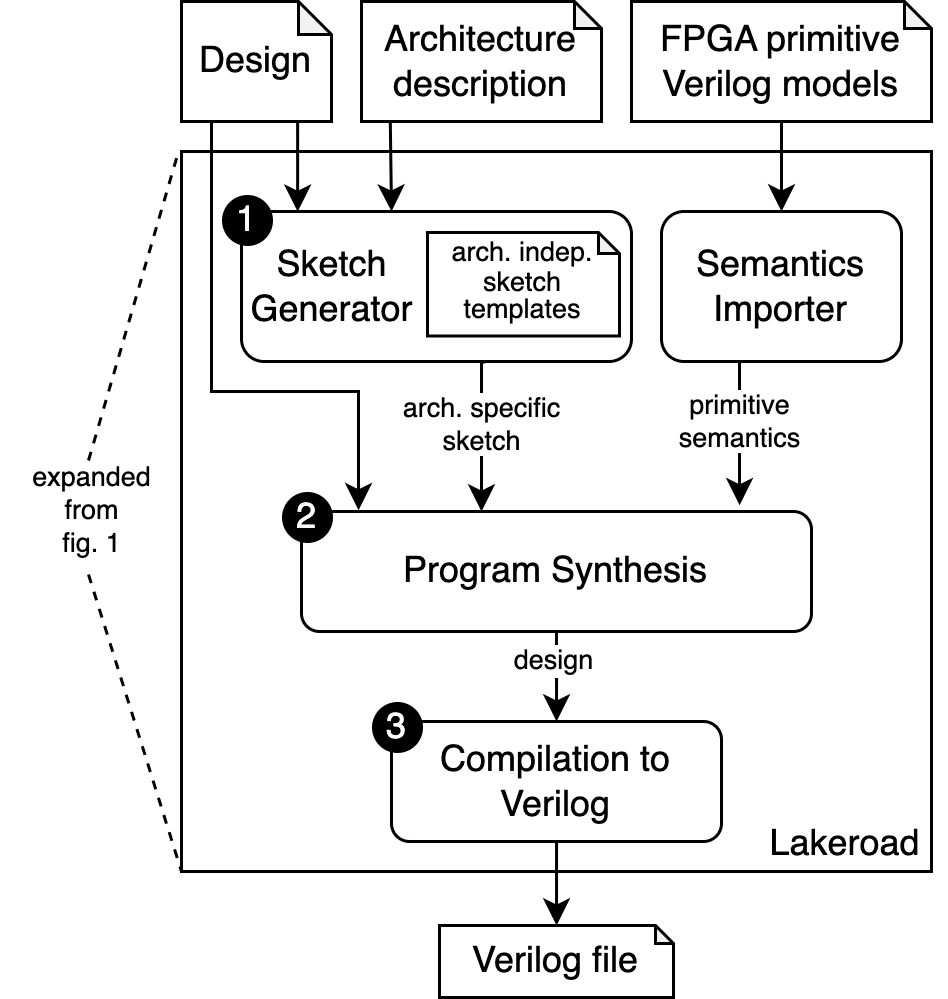
\includegraphics[width=.8\columnwidth]{assets/lakeroad-diagram.drawio.png}
    \caption{\lr system diagram. \hl{instr. spec should be removed, remove design fragment?}}
    \label{fig:lakeroad-diagram}
\end{figure}
  
\cref{fig:lakeroad-diagram}
  illustrates \lr's high-level design.
In this section we discuss the design components,
  and we illustrate \lr's flow with
  an example mapping a MAC (multiply accumulate) onto
  a Xilinx Ultrascale+ DSP48E2.
\hl{change running example to something that doesn't work on Vivado}
  
\lr takes three inputs:
  (1) an \textit{HDL module} specifying
    the FPGA program 
    to be implemented
    for a given architecture,
  (2) an \textit{architecture description} YAML file
    that describes the ports and parameters
    of an architecture's 
    hardware primitives,
  and (3) \textit{vendor-provided Verilog models}
    for the target FPGA architecture.
\hl{Which are user provided?}
\hl{the three inputs come from three different places: hdl model written by user, arch description written by...lakeroad maintainers? and vendor-supplied verilog. This might need a separate sentence.}
% The HDL module is the design which the low-level
%   Verilog will implement.
% The architecture description is a short configuration file
%   describing the ports/parameters of architecture-specific
%   hardware primitives.
% Lastly, the vendor-provided
%   Verilog models correspond to the implementations of
%   architecture-specific primitives
%   (e.g., \texttt{DSP48E2.v} on Xilinx).

These inputs are passed to the \lr pipeline,
  which is responsible for mapping the high-level
  HDL module to an architecture-specific
  implementation.
\cref{fig:firstpage} gives an example
  of \lr's inputs for
  implementing a MAC on a Xilinx
  Ultrascale+ DSP48E2,
  and the resulting
  output.
  
The \lr pipeline consists of
  three main components:
  \textit{sketch generation},
  \textit{program synthesis},
  and \textit{HDL compilation},
  which
  we now describe 
  in greater detail.
 % Together with automated semantics extraction
 %  from vendor-supplied Verilog models of
 %  target FPGA primitives, or manual effort from the user.
  
% \lr takes as input
%   (1) a high-level specification of an instruction,
%   (2) a description of a target FPGA architecture, and
%   (3) vendor-provided Verilog
%   models of the target FPGA's combinational primitives.
% Given these inputs,
%   \lr automatically generates
%   an implementation of the instruction
%   in low-level, architecture-specific
%   Verilog.


\subsection{Sketch Generation}

\lr uses the HDL module and
  the architecture description
  to perform
  \textit{sketch generation}.
Sketch generation
  specializes architecture-independent
  representations of FPGA programs, called
  \textit{sketch templates},
  into architecture-dependent
  \textit{program sketches}.

A \textit{sketch template} specifies
  the \textit{structure}
  of an
  FPGA program
  without specifying
  low-level details;
  rather than describing the concrete
  computations that an FPGA will
  perform, a sketch template describes
  how a program should wire together
  abstract computational components
  called \textit{primitive interfaces}.
In particular,
  sketch templates do \textit{not} specify
  the configurations of programmable
  primitives like LUTs or DSPs. 
Sketch templates also permit 
  some flexibility in wire routing,
  allowing for different common
  wiring patterns
  (e.g., reversing)
  to be explored
  during program synthesis.
\lr
  includes a series of default
  sketch templates,
  but a user can easily add their own if needed.

\hl{Would it be useful to draw parallels 
  between sketches and things similar to sketches
  in existing tools? E.g. Yosys essentially
  has sketches as the right-hand sides of its
  rewrites.}
To synthesize a MAC operation onto a DSP48E2,
  the \texttt{dsp} sketch template would be employed.
  This sketch template is quite simple, and consists of the
  primitive interface of a generic DSP with two inputs and an output.
  The DSP primitive interface does not include any information
  about the internal ports/parameters, as those are architecture-specific.
  
% \lr provides a default set of
%   sketch templates,
%   but a user may
%   define their own
%   if needed.

% In the case of synthesizing a MAC operation,
%   the sketch template would consist of an
%   architecture-agnostic representation of a DSP.
%   The sketch generation process would specialize
%   this template to a representation of a Xilinx-specific
%   DSP.
% \hl{mention how the architecture
%   description gets used here}

Although the \texttt{dsp} sketch template is simple, sketch templates can
  also represent more complex structures of primitives.
  For example, the Bitwise Sketch Template
  captures the structure of
  bitwise operations such as
  bitwise \texttt{\&}
  or bitwise \texttt{|}.
This template takes
  $k$ $n$-bit
  inputs,
  routes the $i$th bit of
  each input
  to a primitive interface
  representing an
  abstract $k$-input LUT,
  and routes the outputs
  of the $i$th LUT primitive
  interface to the $i$th output
  bit. 
  
% Using the provided architecture description,
%   \lr specializes these sketch templates
%   for specific architectures by
%   systematically expanding the abstraction
%   in terms of available primitives,
%   e.g., using a sequence of 4-bit LUTs
%   to concretely implement an abstract 6-bit LUT.
  
% Using sketch templates enables \lr
%   to abstract over common implementation strategies,
%   and thus reuse them across different FPGA architectures,
%   and reduces the input required from the user.
% Sketch templates specialized to an FPGA also serve as the
%   ``sketches'' that Lakeroad leverages during
%   sketch-guided synthesis to fill in.
% Sketches specify the overall structure of
%   a potential low-level implementation,
%   but leave unspecified ``holes'' for
%   LUT, DSP, and carry chain configuration
%   parameters which are then synthesized by
%   a reduction to a sequence of SMT solver queries~\cite{torlak2013growing}.

%\paragraph{(Example) 4-Bit Adder:}
  

% {\it (Example) 4-Bit Adder:}
%   For a more complicated example,
%   consider building a 4-bit binary adder
%   that adds 4-bit bitvectors \texttt{a} and \texttt{b}.
  
% On Xilinx's Ultrascale+ this would
%   be built with four LUT2s,
%   each with configuration
%   \texttt{.INIT(4'h6)} to compute
%   the sum bits,
%   and a CARRY8.
% The outputs of the LUT2s would
%   be wired into the CARRY8's \texttt{.S} ports,
%   and \texttt{a} would
%   be wired into the \texttt{.DI} ports
%   of the CARRY8 to allow carry bit
%   generation.
% On Lattice ECP5 this could be built
%   by connecting 4 CCU2C components
%   into an 8-bit carry chain and connecting
%   8 LUT4s with configuration \hl{specify config}
%   into the carry chain's input.

% On SOFA, which only has LUT4s and does not
%   have a fixed carry-chain unit,
%   the sum bits would be computed with
%   four frac\_lut4s (SOFA's LUT4 primitive) with
%   configuration \texttt{.sram(16'hf77f)}.
%   The outputs of these LUTs as well
%   as one of the inputs (e.g., \texttt{a})
%   would be passed into a complicated
%   carry-chain structure
%   built from frac\_lut4s.
  
% Details differ between architectures but
%   both programs share a common shape:
%   both have four LUTs feeding into a
%   carry chain structure.
% A sketch template captures this
%   similarity by specifying that it wants four LUTs fed
%   into a carry chain.
% It does \textit{not} detail 
%   which FPGA components will be used, or
%   what their configurations will be.\hfill $\qed$

% \hl{is this qed intentional?}

Sketch generation then
  specializes
  sketch templates
  to partially complete
  architecture-specific
  FPGA programs called
  \textit{program sketches}. A program sketch
  contains \textit{holes};
these holes allow flexibility
  in potential program implementations
  and will be filled in later by the Program
  Synthesis component.

% This is repetitive?
A program sketch, like a sketch template, still
  represents the \textit{shape} of an FPGA program
  rather than the program itself:
  while it is now FPGA-specific,
  many of the computational
  components in a program
  sketch are unconfigured,
  and retains the
  same flexibility
  in wire routing
  choices that
  existed in the
  sketch template.
  
With a Xilinx architecture description, sketch
  generation would convert the DSP primitive interface
  to a partially complete representation of the DSP48E2.
  The ports and parameters at this point would be included
  in the representation, but their configuration would
  remain symbolic and need to be solved during Program
  Synthesis.
  
% \lr's templates capture common 
%   implementation patterns
%   used in FPGAs.
% For example,
%   to implement multiple-bit
%   logic operations
%   like 
%   \texttt{a \&\& b}
%   on most FPGAs,
%   the common strategy is to use
%   a one Look-up Table (LUT)
%   per pair of bits,
%   e.g.~\texttt{LUT(a[0], b[0])},
%   \texttt{LUT(a[1], b[1])},
%   and so on.
% Arithmetic operations
%   are implemented similarly,
%   but with an arithmetic carry chain
%   to carry information between bits.
% \lr's templates
%   capture these high-level patterns
%   in an architecture-independent way.

% \lr's templates rely on \textit{primitive interfaces}
%   that represent computations in
%   an architecture-independent way.
% For instance, the LUT-$n$ primitive
%   interface represents
%   an $n$-input 1-output lookup table,
%   and the Carry-$n$ represents an $n$-bit
%   carry chain.
% Architecture descriptions provide implementations
%   for primitive interfaces.
% These implementations may be done with a
%   single hardware primitive
%   or with a combination of hardware
%   primitives.
% \lr also provides logic to perform common
%   primitive combinations, such as
%   recursively building
%   a larger LUT from smaller LUTs.
  

% \textit{Sketch generation}
%   transforms a template to
%   a \textit{sketch}.
% A sketch is a \lrir program with
%   \textit{holes}, or symbolic values
%   that will be later filled in by
%   synthesis to make a concrete \lrir program.
% Sketch generation 
%   queries an
%   \textit{architecture configuration}
%   to find architecture-specific
%   implementations for a
%   template's primitive interfaces.
% These implementations may still be
%   symbolic (that is, they may have holes).

\subsection{Program Synthesis}
\lr uses \textit{sketch-guided program synthesis}~\cite{??}
  to find a low-level, architecture-specific
  FPGA implementation.
Sketch-guided program synthesis is a
  technique that uses a solver
  to look for values to fill in
  a sketch's holes so that it
  implements the specified instruction. For a MAC,
  the end result of program synthesis would be a
  correct configuration of the ports/parameters of
  the DSP48E2 that would implement the operation.

Sketch-guided program synthesis
  requires an interpreter to define
  the semantics of the language that
  the sketch is written in, and
  this usually requires up-front
  investment from
  the user.
This is often a barrier to
  entry and is not an option
  for our use-case.
To avoid this problem, \lr
  \textit{automatically constructs}
  an interpreter by
  (i) providing a base interpreter
  that specifies all
  FPGA-independent semantics
  (e.g., wiring operations, etc),
  and
  (ii) \textit{automatically importing}
  the semantics of FPGA-specific primitives
  from vendor-supplied Verilog models;
A user only
  needs to provide
  a high-level
  description of 
  the target FPGA
  architecture rather
  than explicitly
  writing the interpreter.


This final program will be in \lrir,
  \lr's domain-specific synthesis language.
Both sketch templates and program sketches
  are partial \lrir programs.
  
\subsection{HDL Compilation} 

After program synthesis,
  the \lrir program has filled in all holes
  corresponding to programmable primitive configuration and thus represents a complete low-level design.
Finally, the \lrir program
  is compiled to a HDL that can
  be placed on the physical FPGA.
This compilation is purely syntactic:
  it does no optimization and simply
  maps from one structure to another.
This translation is a simple
  one-to-one correspondence to
  help ensure the correctness
  of the \lrir implementation
  and the compiled HDL program.
For a MAC, this would be a conversion from \lrir to
  the corresponding low-level Verilog.

%\section{\ThePlatonicApproach{} (old)}
%\label{sec:overview}
%
%In this section we introduce \textit{\theplatonicapproach{}}, a novel approach for
%automatically implementing ISA instructions for a target FPGA architecture from
%formal models of the ISA instructions and of  the target architecture.
%%
%\note{Note: I want \theplatonicapproach to include the DSL...THIS IS PART OF THE TECHNIQUE! How do we phrase this?}
%Central to \ThePlatonicApproach is a \textit{customizable} and \textit{extensible} domain specific language (DSL).
%%
%Here is an outline of \theplatonicapproach:
%\begin{itemize}
%    \item A user encodes formal models of each target ISA instruction in the DSL
%    \item The user models \textit{primitives} for the target FPGA architecture by extending the DSL
%    \item \note{are users providing templates/search spaces for the program we are synthesizing? should we be explicit here?}
%    \item \Theplatonicapproach invokes an SMT solver to find a program in the DSL that
%          implements the encoded ISA instruction for the FPGA architecture
%\end{itemize}
%\note{\ldots just a solver? why \textit{constrain}  ourselves (yuk yuk yuk) to SMT solvers?}
%
%\hl{
%System diagram
%
%non-eval contributions explained at a high level
%
%when you finish the overview, you should have an idea of the blocks within lakeroad, but you shouldn't know how they're implemented.
%
%want to mention that it's solver aided
%
%
%what do we care about/what do we want people to continue caring about for the next n years
%
%we want people to care that this is solver-aided
%
%we want people to care that it is user-extensible, to easily support new architectures
%}
%
%\hl{put synthesis statement in overview:}
%FIND \textit{init}\ .\ $\forall a,b,c,d$\ .\  lut(a,b,c,d, \textit{init}) == bvand(a, b)